% Standalone TikZ source for the Fig. 1 method-overview schematic. Pure
% symbolic pipeline diagram -- no result data, nothing to extract/rebuild
% from a frozen JSON (unlike fig1_diorperclass / fig2_covmatched). Notation
% matches \S\ref{sec:methods} exactly (GWD score s(.,.), q-hat, alpha,
% alpha_min, G1/G2 naming, LTT-HB, (beta,delta)). Box text is short labels
% only; the architecture roster and certifiability-floor formulae live in the
% caption (directive #3: no long sentences inside figures).
%
% Single-column span target (IEEE TGRS column width ~3.5in; canonical
% single-column article \textwidth = 6.5in): sized so \includegraphics at
% \columnwidth in TGRS and at native size in the article keeps all box text
% at >=8pt effective at final print size. Compact vertical extent (no towering
% schematic).
\documentclass[tikz,border=1pt]{standalone}
\usepackage[T1]{fontenc}
\usepackage{lmodern}
\usepackage{amsmath,amssymb}
\usetikzlibrary{arrows.meta,positioning,calc}

% Colorblind-safe palette, reused from fig1/fig2 (project's default 8-hue
% categorical theme): seriesGreen for the G1 branch, seriesOrange for the G2
% branch. The detector node reads as an opaque black box via a solid dark
% fill with a light keyline (a bare 100%-black blob reads as a print error;
% the keyline + short label keep the black-box concept legible in print).
\definecolor{seriesGreen}{HTML}{008300}
\definecolor{seriesOrange}{HTML}{EB6834}
\definecolor{boxdark}{HTML}{1A1A1A}

\begin{document}
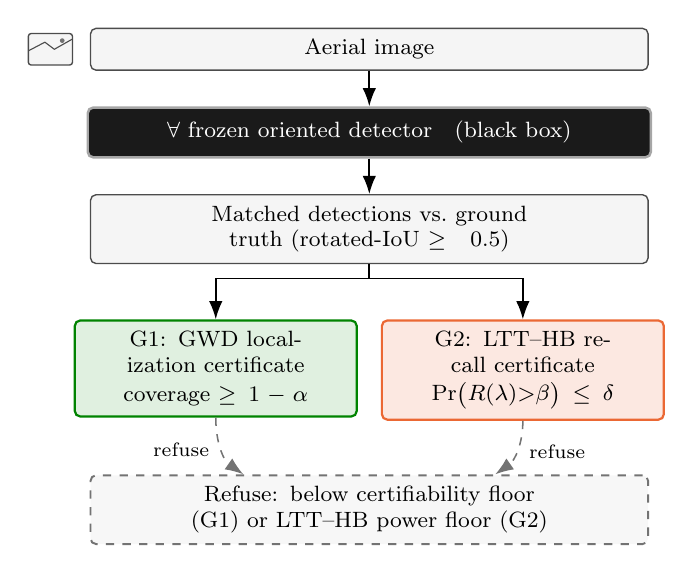
\begin{tikzpicture}[
  font=\fontsize{8}{9.3}\selectfont,
  >={Latex[length=2.3mm,width=1.7mm]},
  node distance=4.5mm,
  pipe/.style={
    rectangle, rounded corners=2pt, draw=black!70, fill=black!4,
    line width=0.5pt, text width=6.8cm, align=center, inner sep=4pt
  },
  blackbox/.style={
    rectangle, rounded corners=2pt, draw=black!35, line width=0.9pt,
    fill=boxdark, text=white, text width=6.8cm, align=center, inner sep=5pt
  },
  g1box/.style={
    rectangle, rounded corners=2pt, draw=seriesGreen, line width=0.8pt,
    fill=seriesGreen!12, text width=3.3cm, align=center, inner sep=4pt
  },
  g2box/.style={
    rectangle, rounded corners=2pt, draw=seriesOrange, line width=0.8pt,
    fill=seriesOrange!15, text width=3.3cm, align=center, inner sep=4pt
  },
  refusebox/.style={
    rectangle, rounded corners=2pt, draw=black!55, dashed, line width=0.7pt,
    fill=black!3, text=black, text width=6.8cm, align=center, inner sep=4pt
  },
  flow/.style={-{>},line width=0.6pt,draw=black},
  refuse/.style={-{>},line width=0.55pt,draw=black!55,dashed},
]

% Small aerial-image glyph (framed photo: horizon + sun), a shape cue rather
% than more text, sitting just left of the input node.
\begin{scope}[shift={(-4.05,0)}]
  \draw[line width=0.5pt, draw=black!70, fill=black!4, rounded corners=1pt]
    (-0.28,-0.2) rectangle (0.28,0.2);
  \draw[line width=0.4pt, draw=black!70] (-0.28,-0.02) -- (-0.07,0.09) -- (0.05,0.0) -- (0.28,0.13);
  \fill[black!55] (0.15,0.11) circle (0.03);
\end{scope}

\node[pipe] (img) {Aerial image};

\node[blackbox, below=of img] (det)
  {$\forall$ frozen oriented detector \; (black box)};

\node[pipe, below=of det] (match)
  {Matched detections vs.\ ground truth (rotated-IoU $\ge 0.5$)};

\node[g1box, below=7mm of match, xshift=-1.95cm] (g1)
  {G1: GWD localization certificate\\[1pt]
   coverage $\ge 1-\alpha$};

\node[g2box, below=7mm of match, xshift=1.95cm] (g2)
  {G2: LTT--HB recall certificate\\[1pt]
   $\Pr\!\big(R(\lambda){>}\beta\big)\le\delta$};

\coordinate (mid) at ($(g1.south)!0.5!(g2.south)$);
\node[refusebox, below=7mm of mid] (refuse)
  {Refuse: below certifiability floor (G1) or LTT--HB power floor (G2)};

\draw[flow] (img) -- (det);
\draw[flow] (det) -- (match);
\draw[flow] (match.south) -- ++(0,-0.18cm) -| (g1.north);
\draw[flow] (match.south) -- ++(0,-0.18cm) -| (g2.north);
\draw[refuse] (g1.south) to[out=270,in=145]
  node[midway, left=1pt, font=\fontsize{7.5}{8.5}\selectfont, text=black] {refuse}
  ($(refuse.north)+(-1.6cm,0)$);
\draw[refuse] (g2.south) to[out=270,in=35]
  node[midway, right=1pt, font=\fontsize{7.5}{8.5}\selectfont, text=black] {refuse}
  ($(refuse.north)+(1.6cm,0)$);

\end{tikzpicture}
\end{document}
